 \subsection{Bah\'ia rectangular de ancho unitario}
  Para validar los resultados de la implementaci\'on del algoritmo, y estudiar la convergencia de \'este, se ha escogido una soluci\'on anl\'itica al problema presentado en la ecuaci\'on \eqref{helmholtz}. Este caso corresponde a una bah\'ia cuadrada de largo unitario cuyo interior es $\Omega = [0,1]\times[0,1]$, la cual se encuentra cerrada por bordes impermeables, es decir, $\partial \Omega_g=0$, y fondo a profundidd $h_0\in\mathbb{R^+}$. Por medio de separaci\'on de variables, al asumir que $u$ puede escribirse como $u(x,y)=f(x)g(y)$, y al considerar las condiciones de borde, se deduce que los modos de oscilaci\'on vienen dados por 
  
  \begin{equation}
    \begin{array}{cc}
    u_{nm}(x,y)=A_{nm}\cos(n\pi x)\cos(m\pi y) & \text{ con } n,m \in \mathbb{N}_0 \text{ y } A_{nm}\in\mathbb{R}
    \end{array}
    \label{eq:bahia_cerrada_modo}
  \end{equation}

  y el per\'iodo de oscilaci\'on asociado
  
  \begin{equation}
    \begin{array}{cc}
    T_{nm}=\dfrac{2}{\sqrt{gh}}\left( n^2+m^2\right)^{-1/2} & \text{ con } n,m \in \mathbb{N}_0
    \end{array}
    \label{eq:bahia_cerrada_periodo}
  \end{equation}
  
Asimismo la longitud de onda queda expresada por: 

  \begin{equation}
    \begin{array}{cc}
    L_{nm}=2 \left( n^2+m^2\right)^{-1/2} & \text{ con } n,m \in \mathbb{N}_0
    \end{array}
    \label{eq:bahia_cerrada_longitud}
  \end{equation}

Se utiliza esta \'ultima, porque permite comparar y verificar directamente con la geometr\'ia de la bah\'ia cuadrada.

La soluci\'on mediante FEM es implementada para distintas resoluciones de malla y su convergencia es estimada calculando el error asociado a la determinaci\'on del valor propio y el vector propio correspondiente, respecto de la soluci\'on anal\'itica. Cabe destacar que los modos propios analizados no son consecutivos debido a la multiplicidad de valores propios al ser una regi\'on con ambas dimensiones equivalentes (ver figura \ref{multiplicidad})

\begin{figure}
  \centering
  \begin{subfigure}{0.3\textwidth}
    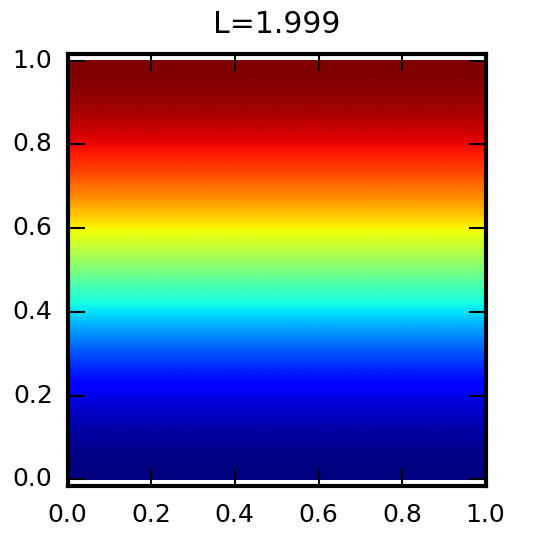
\includegraphics{figuras/modonum_1.png}
  \end{subfigure}
  ~
  \begin{subfigure}{0.3\textwidth}
    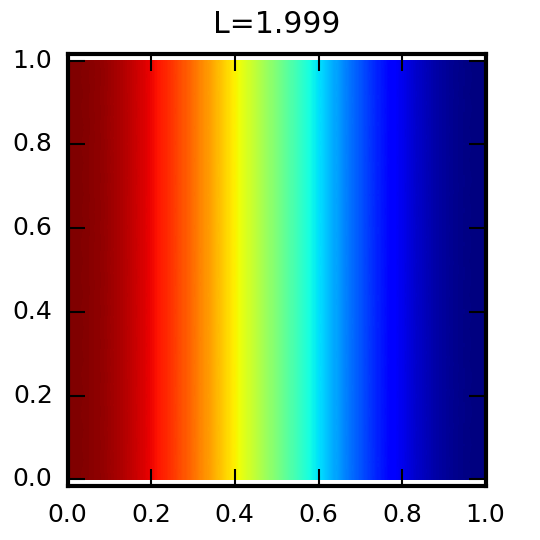
\includegraphics{figuras/modonum_2.png}
  \end{subfigure}
  
  \caption{Ejemplo de la multiplicidad de valores propios: modos de oscilaci\'on 1 y 2 usando $h=1/25$  mediante el m\'etodo de Elementos Finitos.}
\label{multiplicidad}  
\end{figure}

Para la determinaci\'on del error en el valor propio ($E_L$) se utilza norma natural de $\mathbb{R}$

$$E_L = |L^h - L|$$

donde $L$ es la longitud de onda obtenida mediante la soluci\'on anal\'itica $L^h$ es la longitud de onda obtenida mediante aproximaci\'on por FEM.

La figura \ref{fig:valores_propios} muestra los errores como funci\'on de la longitud $h$ del elemento, para los 6 primeros valores propios en cada resoluci\'on de malla. Se verifica que los 6 primeros valores propios se aproximan de manera ordenada a los valores propios de la soluci\'on anal\'itica.

\begin{figure}
  \centering
  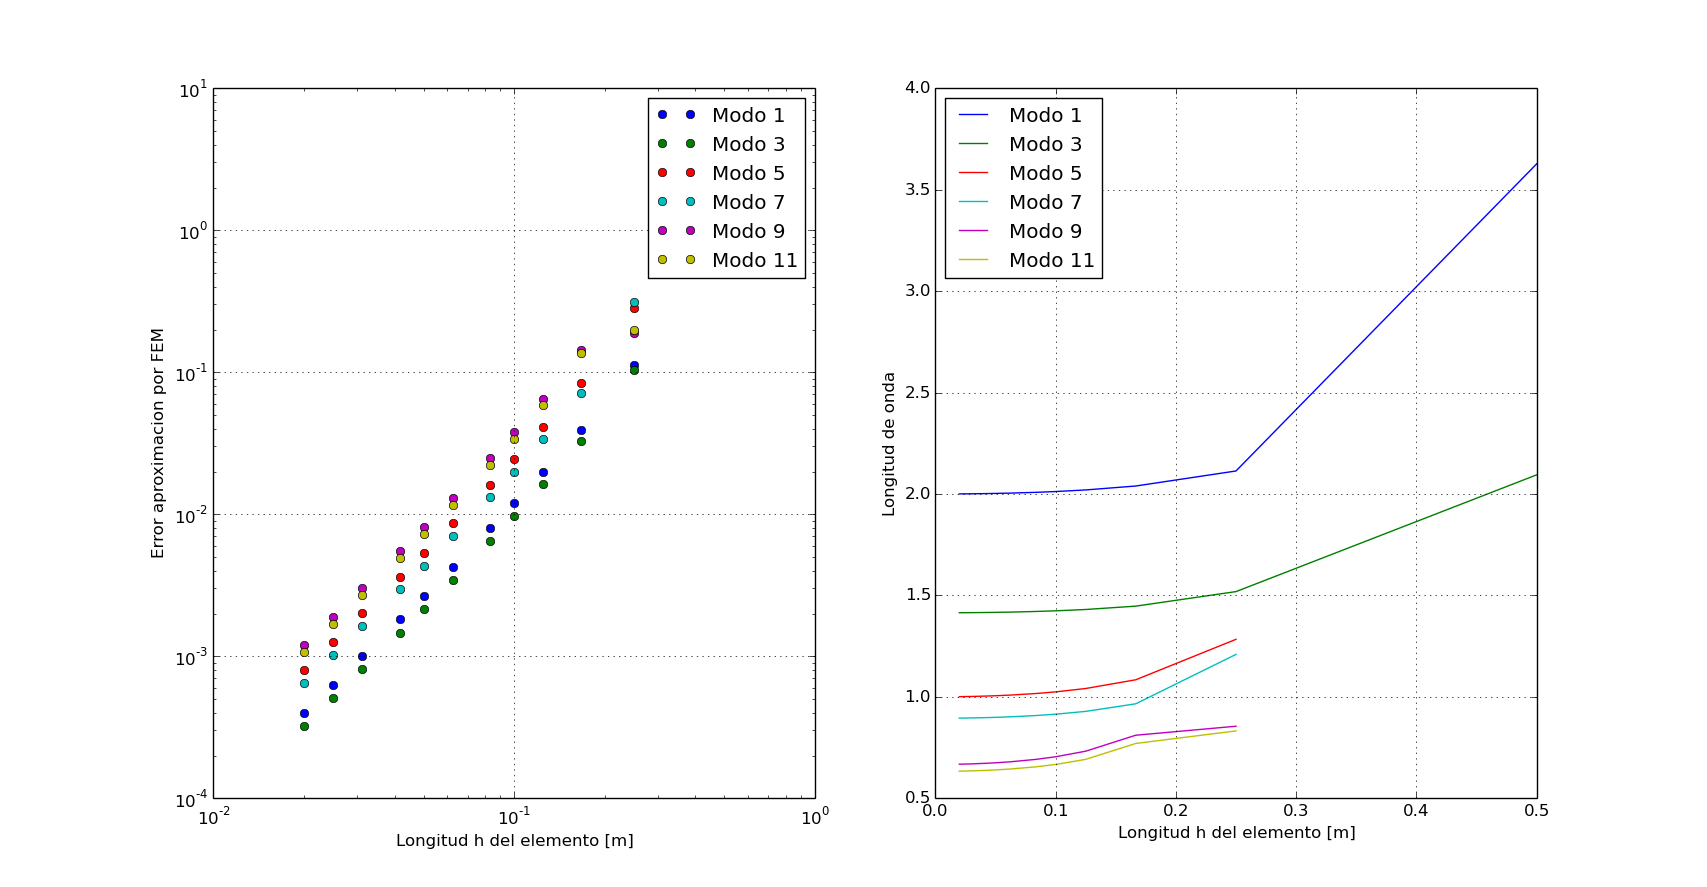
\includegraphics[width=17cm]{figuras/valores_propiosFEM.png}
  \caption{ Resultados aproximaci\'on valores propios mediante FEM y errores asociados}  
  \label{fig:valores_propios}
\end{figure}

Para estimar el orden de convergencia se ajusta una curva a los datos ($log(E)$, $log(h)$) para cada resoluci\'on de malla, ajustando una recta $log(E) = log(C) + p log(h)$ donde p nos indica la taza de convergencia.

La siguiente tabla muestra los resultados de convergencia para los 6 primeros modos.

\begin{table}[h]
\centering
\begin{tabular}{|c|c|c|}
\hline 
Modo & C & p \\ 
\hline 
1 & 0.62007961 & 2.4403783 \\
\hline 
3 & 0.39830035 & 2.33894099 \\ 
\hline 
5 & 0.69813644 & 2.26494859 \\  
\hline 
7 & 0.71017628 & 2.33846474 \\ 
\hline 
9 & 0.68486822 & 2.12311422 \\  
\hline 
11 &  0.70325574 & 2.17136287 \\
\hline 
\end{tabular} 
\caption{Coeficientes del ajuste de las curvas $\log(E_L)=\log(C)+p\log(h)$} para los 6 primeros modos.
\label{tabla:EL}
\end{table}

Para el caso del error de los vectores propios (que corresponde a la desnivelaci\'on instant\'anea), este se calcula mediante la norma de $\mathcal{L}^2(\Omega,\mathbb{R})$

$$E_u = \left(\int_{\Omega} (u^h - u) \mathrm{d}\boldsymbol{x} \right)^{1/2}$$

Los resultados obtenidos para cada resoluci\'on de malla se muestran en la figura \ref{fig:vectores_propios}.

\begin{figure}
  \centering
  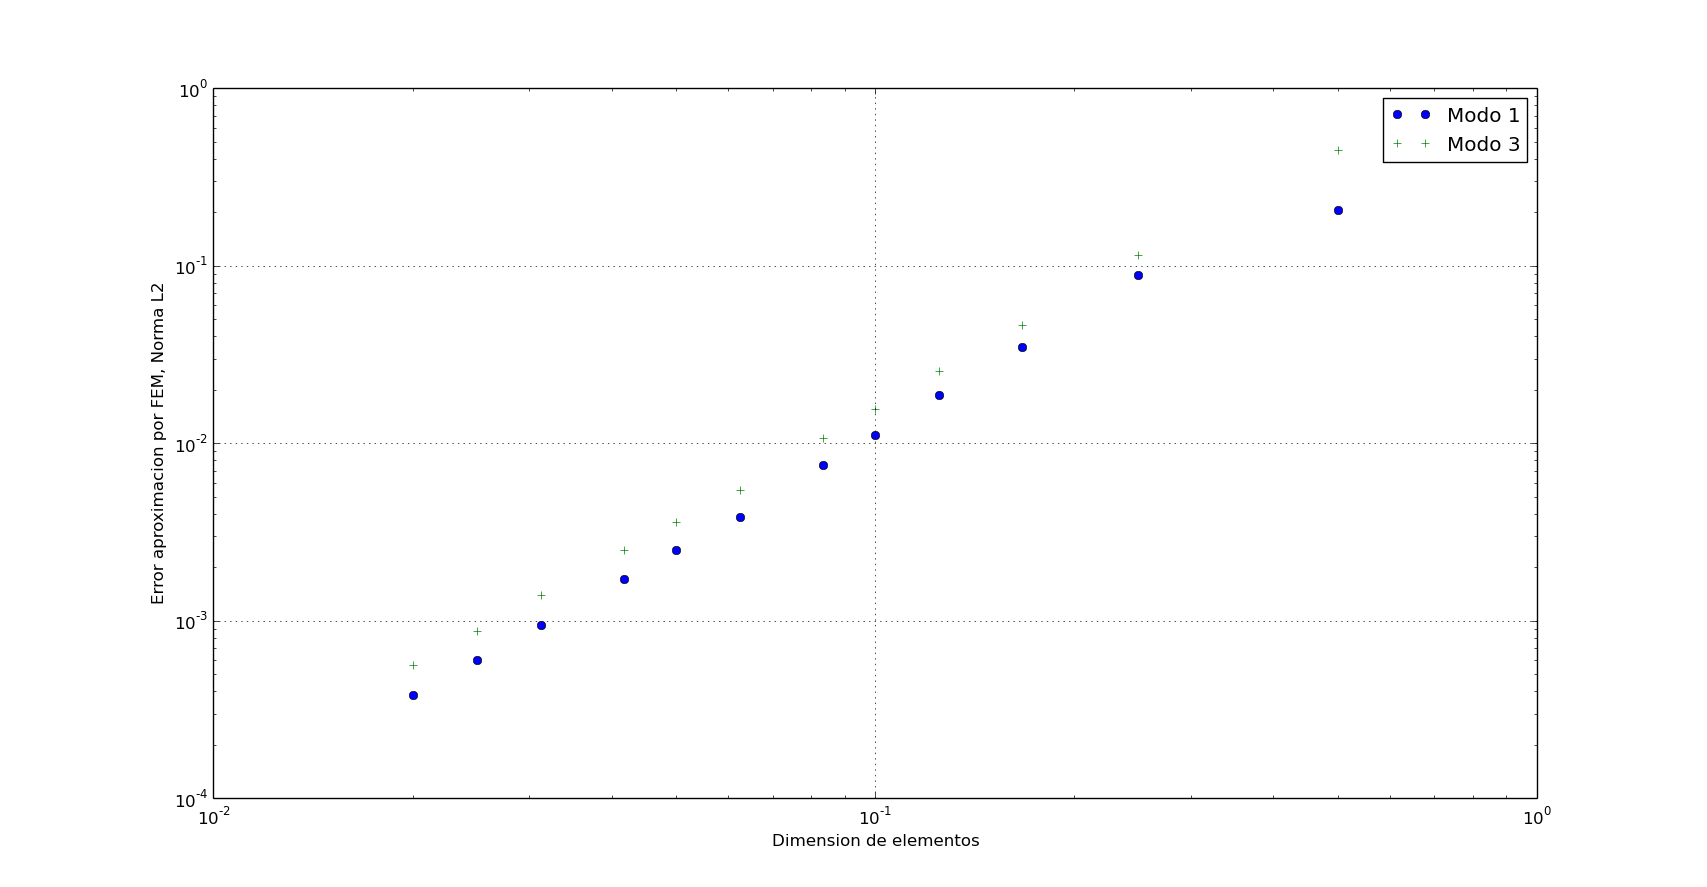
\includegraphics[width=17cm]{figuras/vectores_propiosFEM.png}
  \caption{Errores en norma $\mathcal{L}^2$ de los vectores asociados a cada modo propio}
  \label{fig:vectores_propios}
\end{figure}

Para estimar la taza de convergencia se ajusta una curva a los datos ($log(E_u)$, $log(h)$), de manera similar a los valores propios. Los resultados para los dos primeros modos se muestran la siguiente tabla. Es importante señalar que para estimar el error se debe escalar los resultados de FEM, pues en la soluci\'on anal\'itica se utiliz\'o una amplitud m\'axima de 1 con valores positivos en el borde izquierdo. En ambos casos se puede ver que la taza de convergencia es de orden 2.

\begin{table}
  \centering
  \begin{tabular}{|c|c|c|}
  \hline 
  Modo & C & p \\ 
  \hline 
  1 & 0.0765871 & 2.04894336 \\  
  \hline 
  3 & 0.29036431 & 2.09300275 \\  
  \hline 
  \end{tabular} 
  \caption{Coeficientes de ajuste de las curvas $\log(E_u)=\log(C)+p\log(h)$}
  \label{tabla:Eu}
\end{table}


\begin{figure}
  \centering
  \begin{subfigure}{0.4\textwidth}
    \centering
    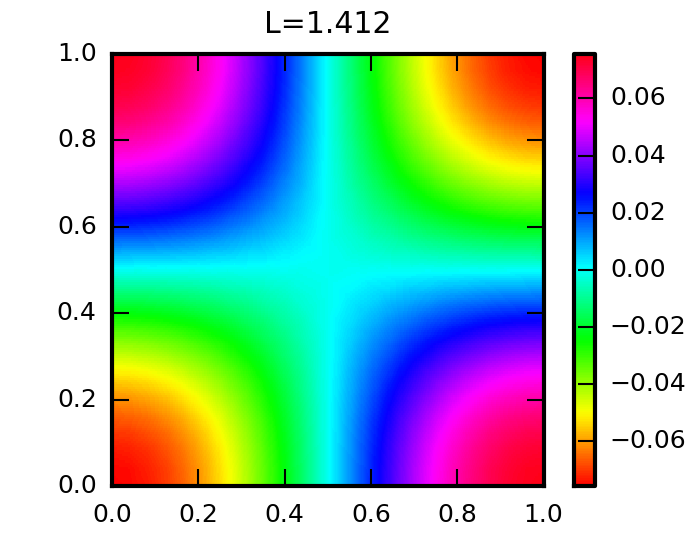
\includegraphics{figuras/modonum_3.png}
  \end{subfigure}
  ~
  \begin{subfigure}{0.4\textwidth}
    \centering
    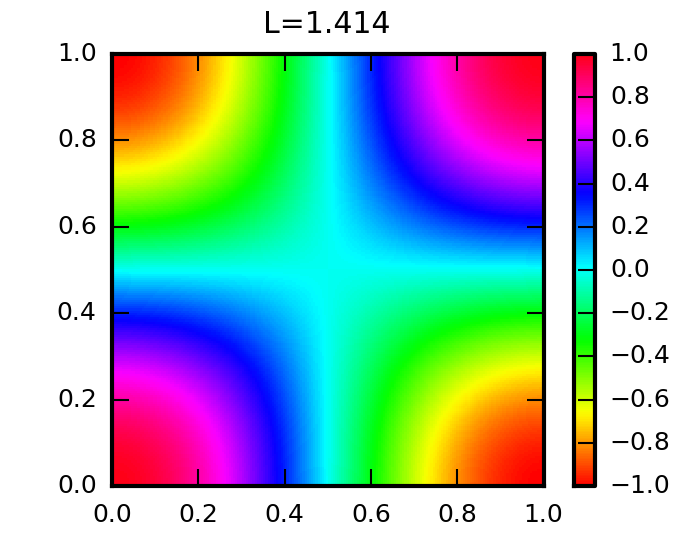
\includegraphics{figuras/modoanalitico_1_1.png}
  \end{subfigure}
  
  
  \begin{subfigure}{0.4\textwidth}
    \centering
    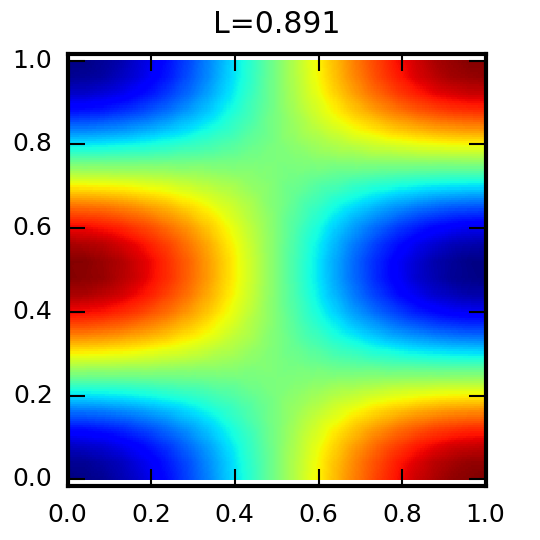
\includegraphics{figuras/modonum_6.png}
  \end{subfigure}
  ~
  \begin{subfigure}{0.4\textwidth}
    \centering
    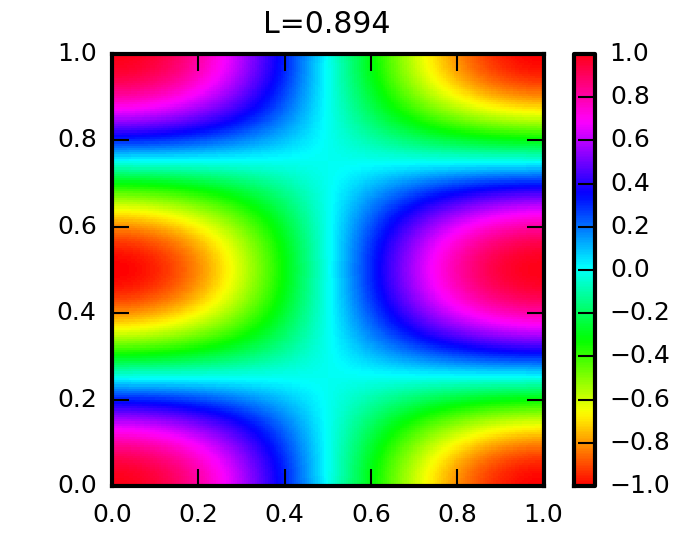
\includegraphics{figuras/modoanalitico_1_2.png}
  \end{subfigure}   
  \caption{Modos de oscilaci\'on 3 y 6 obtenidos num\'ericamente para $h=1/25$ (primera columna) y mediante la soluci\'on anal\'itica para $(n,m)=(1,1)$ y $(n,m)=(1,2)$ (segunda columna)}
  \label{fig:modos_numericovsanalitico}
\end{figure}

